\documentclass[conference]{IEEEtran}
\IEEEoverridecommandlockouts

\usepackage{amsmath,amssymb,amsfonts}
\usepackage{graphicx}
\usepackage{booktabs}
\usepackage{array}
\usepackage{url}
\usepackage{textcomp}
\usepackage{xcolor}
\usepackage{enumitem}

% ---- space levers (typographic only; no content changed) ----
\setlist{itemsep=0pt,parsep=0pt,topsep=2pt,partopsep=0pt}
\setlength{\abovedisplayskip}{3pt}
\setlength{\belowdisplayskip}{3pt}
\setlength{\abovedisplayshortskip}{2pt}
\setlength{\belowdisplayshortskip}{2pt}

\graphicspath{{figs/}}

% ---- manual figure/table caption helpers (arabic numbering to match prose) ----
% We typeset captions as plain paragraphs so the numbers in the prose
% ("Table 3", "Figure 2", "Table B1") always match, avoiding IEEEtran's
% Roman auto-numbering. No \caption is used.
\newcommand{\floatcap}[1]{{\footnotesize\itshape #1\par}}

\begin{document}

\title{End-to-End Coupling Is the Wrong Default for\\ Inductive Temporal Link Prediction}

\author{%
\IEEEauthorblockN{Duong Viet Hoang\textsuperscript{*}}
\IEEEauthorblockA{Department of Computer Science\\
Da-Yeh University, Taiwan\\
Hoangduong4316@icloud.com\\
\textsuperscript{*}Corresponding author}
\and
\IEEEauthorblockN{Duong Viet Huy}
\IEEEauthorblockA{Department of Computer Science\\
Kent State University, United States\\
huydv6210@gmail.com}
\and
\IEEEauthorblockN{Lun-Min Shih}
\IEEEauthorblockA{Department of Computer Science\\
Da-Yeh University, Taiwan\\
Lmshih@mail.dyu.edu.tw}
}

\maketitle

\begin{abstract}
Temporal link predictors are trained end-to-end: the link loss shapes the representation. We show this near-universal default is the wrong one for \emph{inductive} generalization, and that the damage it does is irreversible. Our instrument is a temporal architecture whose continuous backbone (an event encoder, a multi-signal per-pair edge-state operator, and a coupled-GRU memory) can be run with the link gradient either reaching it or stopped at a single point, holding everything else fixed. Flipping that one switch is decisive: enabling the end-to-end link head, every other setting fixed, drops inductive average precision (AP) on CoEdit (a co-edit graph we introduce) by 21.1 points (0.9899 $\rightarrow$ 0.7788), which is essentially the entire decoupled-vs-coupled gap. The same single change keeps decoupling ahead on two standard graphs we did not build (Wikipedia +4.9, MOOC +0.9), so the mechanism is not a CoEdit artifact. At five seeds the decoupled model reaches 0.9876 inductive AP, +22.8 over the coupled variant, and leads a protocol-matched TGAT by +14.1 \emph{within our shared harness}. Our baselines are simplified re-implementations, so this is a within-harness margin, not a claim against published state of the art ($\S$4.1). The primitives are prior art (stop-gradient, frozen probing); the finding is not. A decisive control shows classic freeze-then-probe reaches only 0.768 (CoEdit) and 0.951 (Wikipedia), landing beside the coupled arm, whereas decoupling-by-construction reaches 0.988 / 0.998: once the link loss has shaped the backbone, freezing it and re-probing recovers nothing. To our knowledge this irreversibility is new for temporal link prediction; the prescription is to prevent the contamination by construction, and the tax it removes is localized to the inductive split. Under both historical and inductive hard negatives [Poursafaei et al., 2022] the ordering does not invert but widens to +40--43 points on Wikipedia and CoEdit, as the coupled arm collapses toward chance. A companion study builds a faithful, intervene-able symbolic lifecycle readout on top of the same decoupled representation, at zero cost to the accuracy result reported here.
\end{abstract}

\begin{IEEEkeywords}
Inductive temporal link prediction, regularization by decoupling, stop-gradient feature decoupling, temporal graph neural networks, information bottleneck, reproducible evaluation.
\end{IEEEkeywords}


\section*{1.~~Introduction}

Temporal interaction graphs are sequences of timestamped edges. Formally, a stream is an ordered event set \(\mathcal{E} = \{(u_i, v_i, t_i, x_i)\}_{i=1}^{N}\), \(t_1 \le \dots \le t_N\), with optional edge feature \(x_i\). The canonical task is \emph{future link prediction}: given history \(\mathcal{H}_t\), score whether a candidate edge \((u, v)\) occurs at \(t\); the model outputs \(\hat{p} = \sigma(f_\theta(u, v, t, \mathcal{H}_t))\) trained by BCE against observed positives and sampled negatives.

Two protocols reward different inductive biases. \textbf{Transductive} test edges reuse training nodes, so a model can lean on a memorized per-node embedding. \textbf{Inductive} test edges involve a node unseen in training, so any per-node embedding is uninitialized at test time. Inductive is the deployment-relevant and harder regime: the model must score from \emph{transferable} dynamics rather than node identity. A model that wins transductively but collapses inductively has memorized the population, not learned the process.

State-of-the-art methods are \emph{memory} models (JODIE, TGN, DyRep) or \emph{encoder} models (TGAT, CAWN, GraphMixer); both train the representation \emph{end-to-end} against the link objective ($\S$2). This has a direct cost we isolate in this paper: with write access to the backbone, gradient descent encodes features that merely \emph{identify} training nodes---rewarded transductively, dead weight inductively. A second cost of end-to-end training is opacity (a node-memory vector cannot easily be interrogated about \emph{why} it scores a pair the way it does), which is not this paper's subject; a companion study shows that the same architectural change we study here also enables a cheap, faithful interrogation mechanism, but we do not repeat that result.

To test that cost we need an architecture in which the link gradient can be admitted to, or withheld from, the representation at a single well-defined point, with everything else held fixed. We build one. It keeps a rich continuous backbone (an event encoder, a multi-signal per-pair edge-state operator grounded in Hawkes intensity [Hawkes, 1971], and a coupled-GRU node-memory module) but \textbf{decouples it from the link loss by an explicit stop-gradient} on the backbone's per-pair representation \(h_{uv}\). The backbone is then shaped only by a variational parsimony objective (a KL regularizer in the spirit of the information bottleneck [Tishby et al., 2000] and the VAE [Kingma \& Welling, 2014]) plus deterministic update laws, and a lightweight symbolic head reads this \emph{frozen} representation to produce the scored edge-existence logit, a stop-gradient device of the kind that stabilizes siamese learning against shortcut collapse [Chen \& He, 2021]. $\S$3 gives the gradient routing. The architecture is the measurement instrument here, not the product: what we are selling is the finding it isolates, and the prescription that follows from it.

Our contributions are:

\begin{enumerate}
\item \textbf{Regularization-by-decoupling for inductive temporal link prediction (core result).} The building blocks (stop-gradient [Chen \& He, 2021], frozen probing [Alain \& Bengio, 2017; Kumar et al., 2022], the information bottleneck [Tishby et al., 2000]) are prior art. We establish, by a single-variable ablation and an irreversibility control, that \textbf{end-to-end coupling is the wrong default for inductive temporal link prediction, and that the damage it causes is irreversible}. Freeze-then-probe cannot recover it. To our knowledge this irreversibility has not previously been shown in this setting. (a) A single-variable three-seed ablation isolates the cause: enabling the end-to-end link head, every other setting fixed, costs \textbf{$-$21.1 points} inductive AP on CoEdit (0.9899 $\rightarrow$ 0.7788), essentially the entire decoupled-vs-coupled gap, with two co-varying readout settings inert ($\S$4.2). (b) The same single change keeps decoupling ahead on two \emph{standard} graphs we did not construct (Wikipedia +4.9 pp, MOOC +0.9 pp), so the mechanism is not a CoEdit artifact, its magnitude tracking how much node identity the coupled head can exploit ($\S$4.4). (c) A decisive control measures the delta against freeze-then-probe: freezing the backbone \emph{after} the link loss reaches only 0.768 (CoEdit) and 0.951 (Wikipedia)---beside the coupled end-to-end arm, far below the 0.988 / 0.998 of decoupling-by-construction---so the damage is \textbf{irreversible} on both datasets, and the contribution is preventing that contamination by construction ($\S$4.2). With no link-prediction gradient the backbone keeps a generic per-pair representation that transfers to unseen nodes, and the identity-shortcut tax it removes lands almost entirely on the inductive split ($\S$5).
\item \textbf{The architectural component that makes the measurement possible: a multi-signal per-pair edge-state operator} (Hawkes intensity, Welford gap statistics, recurrence and rate EWMAs) with a \emph{read-before-write} batched estimator that fixes a silent intra-batch staleness bug. This is a real architectural contribution in its own right---the fix is AP-positive (+5.7 pp inductive in the decoupled model, $\S$3.2)---but its role in this paper is instrumental: it gives the backbone enough per-pair signal that the decoupled representation is a serious competitor, so that withholding the link gradient is a fair test rather than a handicap.
\end{enumerate}

Building on this decoupled representation, a companion study develops a faithful, intervene-able symbolic readout of the per-pair lifecycle; we do not repeat that contribution here.

We measure the decoupled model against a field of competitors on CoEdit (parametric temporal-GNN families, two EdgeBank memorization floors [Poursafaei et al., 2022], and the transformer DyGFormer [Yu et al., 2023]) through one leak-audited harness at three seeds ($\S$4.1).

\section*{2.~~Related work}

\textbf{Memory-based temporal GNNs.} JODIE [Kumar et al., 2019], TGN [Rossi et al., 2020] and DyRep [Trivedi et al., 2019] all maintain a per-node recurrent state trained end-to-end against the link objective (JODIE co-evolves user/item RNNs with a trajectory projection; TGN adds graph-attention over a node-memory; DyRep is a temporally-attentive point process). The architecture we study also carries memory (a coupled-GRU node-memory module) but shapes it by a parsimony objective rather than the link loss, which is exactly the difference our ablation isolates.

\textbf{Encoder, walk, and transformer methods.} TGAT [Xu et al., 2020] self-attends over the temporal neighborhood with a Bochner time encoding, giving native inductive support without a stored node state. CAWN [Wang et al., 2021] encodes anonymized causal walks; GraphMixer [Cong et al., 2023] replaces attention with a token-mixing MLP. The recent inductive frontier adds TCL [Wang et al., 2021b] (contrastive neighborhood representations), NAT [Luo \& Li, 2022] (dictionary-based neighbor features), and \textbf{DyGFormer} [Yu et al., 2023] (a co-occurrence-encoding patching transformer, current temporal-graph-transformer SOTA). We run DyGFormer through our harness on CoEdit, Wikipedia, and MOOC ($\S$4.1); TCL and NAT are not yet run on any dataset, so our frontier comparison is \textbf{partial}, and we downscope the positioning accordingly ($\S$6.2) rather than claim to beat the full named frontier. TGAT is a telling case for the argument of this paper: it self-attends over identity-bearing node features and, on a Wikipedia graph whose user and item id spaces were accidentally merged, scored near-perfect inductive AP; once the id spaces are made correctly disjoint (Appendix A) its inductive AP falls to 0.733, exactly the identity-shortcut failure a coupled representation is prone to ($\S$5).

\textbf{Benchmarks, fair evaluation, and memorization floors.} Poursafaei et al.~[2022] show much of the apparent skill of parametric temporal models is matched by \textbf{EdgeBank}, a non-parametric heuristic predicting an edge if the pair was ever (or recently) seen, and argue any headline must beat this floor under harder negatives; the Temporal Graph Benchmark [Huang et al., 2023] shows rankings reorder under a fair protocol. We adopt both: every model (including two EdgeBank variants) runs through one shared harness with a single negative pool and a leak-audited evaluator, both protocols reported, the floor \emph{measured} (Table 1).

\textbf{Decoupling, frozen representations, and stop-gradient as regularizers.} This paper sits at the intersection of stop-gradient against collapse (SimSiam [Chen \& He, 2021]), frozen-encoder linear probing [Alain \& Bengio, 2017] where fine-tuning can distort transferable features so a probe transfers better [Kumar et al., 2022], and gradient-stopping as capacity control [Caron et al., 2021], readable through the information bottleneck [Tishby et al., 2000; Alemi et al., 2017]. These primitives are prior art, and ``freeze a pretrained encoder, probe with a task head, gain transfer'' is a known phenomenon. Our delta over them is sharp on two fronts. First, \textbf{relocation}: we move stop-gradient-as-regularizer into the \emph{inductive split of temporal link prediction}, where end-to-end coupling is the universal default---and we measure, for the first time in this setting, that coupling is the wrong default. Second, \textbf{isolation}: the backbone is trained only by a parsimony objective from scratch (the regime is task-gradient-vs-none, not pretrain-then-probe), and we localize the tax to an identity shortcut that lands almost entirely on the inductive split ($\S$5). This sharpens the nearest neighbor (Kumar et al.'s ``fine-tuning distorts transferable features'') into a stronger, measured claim: the distortion is \emph{irreversible}. Freezing the backbone \emph{after} the link loss does not recover it, on two datasets ($\S$4.2). The contribution is never exposing the backbone to the link gradient in the first place.

\textbf{Positioning.} We do not claim a new state-of-the-art model: the architecture we build is not the first memory model, nor the first to use Hawkes intensities, and we do not enter it into a leaderboard fight it would not be equipped to win ($\S$6.4). The claim is the \emph{measurement}: \textbf{decoupling} the representation from the link loss is what makes a per-pair dynamical representation generalize inductively, and no post-hoc freezing substitutes for it. A companion paper builds a faithful, intervene-able symbolic readout on the same decoupled backbone; that readout is an add-on this paper does not need to establish the decoupling result.

\section*{3.~~Method}

\subsection*{3.1~~Two streams, one stop-gradient}

The architecture is a two-stream model. Let an event be a timestamped edge \((u, v, t)\) with optional feature vector \(x\).

\textbf{Stream A: continuous backbone.} An \textbf{event encoder} (a residual continuous-signal network) maps event features and source staleness \(\Delta t = t - t_{\text{last}}(u)\) to a per-event representation \(e_{uv}\). A multi-signal \textbf{edge-state operator} maintains, per ordered pair \((u,v)\), a small bank of running statistics:

\begin{itemize}
\item a \textbf{Hawkes self-exciting intensity} \(\lambda_{uv}\) updated at each event by \(\lambda \leftarrow 1 + (\lambda - 1)\,e^{-\beta \Delta t}\), so each interaction transiently raises the pair's rate and the rate decays between events;
\item \textbf{Welford online mean and variance} of the inter-event gap, updated by the numerically-stable recurrence \(\mu_k = \mu_{k-1} + (g_k - \mu_{k-1})/k\), \(M_k = M_{k-1} + (g_k - \mu_{k-1})(g_k - \mu_k)\), with \(\sigma_k^2 = M_k/k\) [Welford, 1962];
\item a \textbf{recurrence EWMA} counting repeated co-occurrence, and \textbf{fast/slow rate EWMAs} \(r^f, r^s\) whose ratio \(r^f/r^s\) is a rising-vs-falling cadence signal;
\item a \textbf{leaky rate-peak} that tracks the maximum recent rate with slow decay.
\end{itemize}

A \textbf{coupled-GRU memory module} updates per-node memory \(m_u, m_v\) from \(e_{uv}\) and emits a parsimony KL term \(\mathrm{KL}(q(z \mid m) \,\|\, p(z))\). The backbone's \emph{only} training signal is this KL (weighted by \(\lambda_{\text{kl}}\)) plus the deterministic update laws above; \textbf{no link-prediction gradient reaches it.}

\textbf{Stream B: symbolic readout (summary).} From the stop-gradiented edge representation \(h_{uv}\), a lightweight symbolic module produces a per-pair lifecycle state over five phases---IDLE, BIRTH, REINFORCE, DECAY, DEATH---and a next-state distribution, shaped by a fixed causal admissibility structure over transitions; an existence decoder maps this distribution to the edge-existence logit that is \textbf{scored}. The decode-tree design, the calibration objective, and the module's use as a faithful, intervene-able readout are developed in a companion paper. The only property this paper's core result depends on is that the decoder is a deterministic, differentiable function of the frozen representation, so no gradient path through it can reach the backbone.

\textbf{The stop-gradient.} The input to every Stream-B module is \(\mathrm{sg}[h_{uv}]\). The scored logit is the existence-decoder logit, and every path from it to the backbone crosses a stop-gradient. A \textbf{gradient-ancestry test} ($\S$3.3) confirms that back-propagating the prediction loss deposits exactly zero gradient on every backbone tensor. A non-stop-gradiented predictor head exists in the implementation but is used only for the end-to-end \emph{ablation} ($\S$4.2).

\subsection*{3.2~~The per-pair operator and the read-before-write estimator}

The operator must read each pair's \emph{pre-event} statistics: scoring event \(i\) may use only state from events \(j < i\), or evaluation leaks the label. A naive batched store snapshots state once per minibatch, so repeated same-pair events \emph{within} a batch read the same stale row and only the last write persists. At batch size 500 on CoEdit the Welford count capped near 6 even for pairs editing 200+ times, silently disabling the DECAY-vs-REINFORCE distinction, which is read off a rate ratio that never accumulated.

The \textbf{read-before-write estimator} replays the deterministic channels event-by-event in stream order, so the \(k\)-th in-batch occurrence reads the post-state of the \((k{-}1)\)-th while scoring stays strictly pre-update (no re-leak; it matches a batch-size-1 reference to max \(|\Delta|=0.000\)). The fix is \textbf{AP-positive}: in the decoupled model it lifts inductive AP 0.9312 $\rightarrow$ 0.9885 (\textbf{+5.7 pp}, three seeds) and transductive +0.65 pp, because the previously-collapsed statistics are exactly the ones the readout decoder reads.

\subsection*{3.3~~The decoupling, exactly}

The total loss is
{\small
\[
\mathcal{L} = \underbrace{\mathcal{L}_{\text{BCE}}(\hat{p}, y)}_{\text{prediction}} + \lambda_{\text{kl}}\,\mathrm{KL}\big(q(z\mid m)\,\|\,p(z)\big) + \lambda_{\text{dc}}\,\mathcal{L}_{\text{decol-CE}}(s_{t+1}^{\text{cal}}) ,
\]}%
with three disjoint gradient routes: the \textbf{backbone} receives only the parsimony KL and deterministic laws; the \textbf{existence head} (scored \(s^{\text{pos}}_{t+1}\) path) only \(\mathcal{L}_{\text{BCE}}\); the \textbf{hierarchical readout heads} (interpretable \(s^{\text{cal}}_{t+1}\) path, detailed in the companion paper) only \(\mathcal{L}_{\text{decol-CE}}\). The stop-gradient on \(h_{uv}\) blocks every Stream-B gradient from the backbone, so both heads read a frozen representation and the auxiliary objective leaks nowhere.

We verify this by a \textbf{gradient-ancestry test} rather than by inspection. On a trained decoupled model over a 1,500-edge CoEdit subsample, we back-propagate the prediction loss alone and let autograd determine which parameters are reached; the set of parameters receiving nonzero gradient is required to be a subset of the scored-head parameters. The test is name-independent (it does not iterate over a heuristically labelled backbone subset, so a backbone tensor cannot be silently skipped) and it passes with \textbf{max \textbar backbone gradient\textbar{} \(= 0.000\mathrm{e}{+}00\)} and an empty set of nonzero backbone tensors: no parameter outside the scored existence head receives any prediction-loss gradient.

\section*{4.~~Experiments}

\subsection*{4.1~~Cross-dataset, protocol-matched, three seeds}

Throughout, \textbf{the decoupled model} (``Decoupled (ours)'' in tables) denotes the proposed configuration of $\S$3 (stop-gradiented backbone, multi-signal edge-state operator, symbolic lifecycle readout, causal readout policy) and \textbf{the coupled model} (``Coupled (end-to-end)'' in tables) denotes an otherwise-identical variant whose link head trains the backbone end-to-end. The two differ only in where the link gradient is allowed to go.

\textbf{The CoEdit benchmark.} CoEdit is a \textbf{non-bipartite co-edit interaction graph}: nodes are contributors, edges are timestamped co-edit events between two contributors on the same artifact, so \emph{both} endpoints carry a lifecycle (unlike the bipartite Wikipedia/MOOC graphs). It uses the same 70/15/15 chronological split and leak-audited negative pool as the standard datasets (construction protocol and statistics in Appendix A). The +13.5 headline is CoEdit-specific ($\S$6.1).

All models run through the \textbf{same} harness, splits, and leak-audited negative pool ($\S$4.3 confirms test AP is not 1.0), built fairly per protocol: transductive negatives are drawn seen$\rightarrow$seen and inductive negatives from the unseen-node pool, so an inductive positive is never scored against a trivially-impossible negative. AP is the standard \texttt{average\_precision\_score} implementation for every model. Every cell is mean $\pm$ sample std over seeds \{1, 7, 42\}; MOOC baselines were re-run on the same seed set so that every model in Tables 1-2 shares it. The decoupled model is tuned on CoEdit only.

\textbf{The CoEdit competitor set.} Nine competitors run through the same harness on CoEdit (Tables 1-2): six parametric temporal-GNN families, two EdgeBank memorization-floor variants [Poursafaei et al., 2022], and the inductive-frontier transformer DyGFormer [Yu et al., 2023]. ``+13.5'' is over the best \emph{measured} CoEdit competitor (TGAT, 0.853); we do \textbf{not} claim to beat the full named frontier: TCL/NAT are unrun, so the frontier comparison is partial ($\S$6.2).

\textbf{Is CoEdit pessimizing baselines specifically?} No.~Our simplified DyGFormer re-implementation is below its published level on \textbf{Wikipedia} as well (0.786 here vs $\approx$0.98 published; the gap is architectural, see the baseline-fidelity note after Table 1), so its low CoEdit AP is the re-implementation ceiling, not CoEdit-specific starvation. What we read from Tables 1-2 is the \emph{relative} ordering within one shared harness; the absolute levels are not comparable to published SOTA.

\begin{figure}[t]
\centering
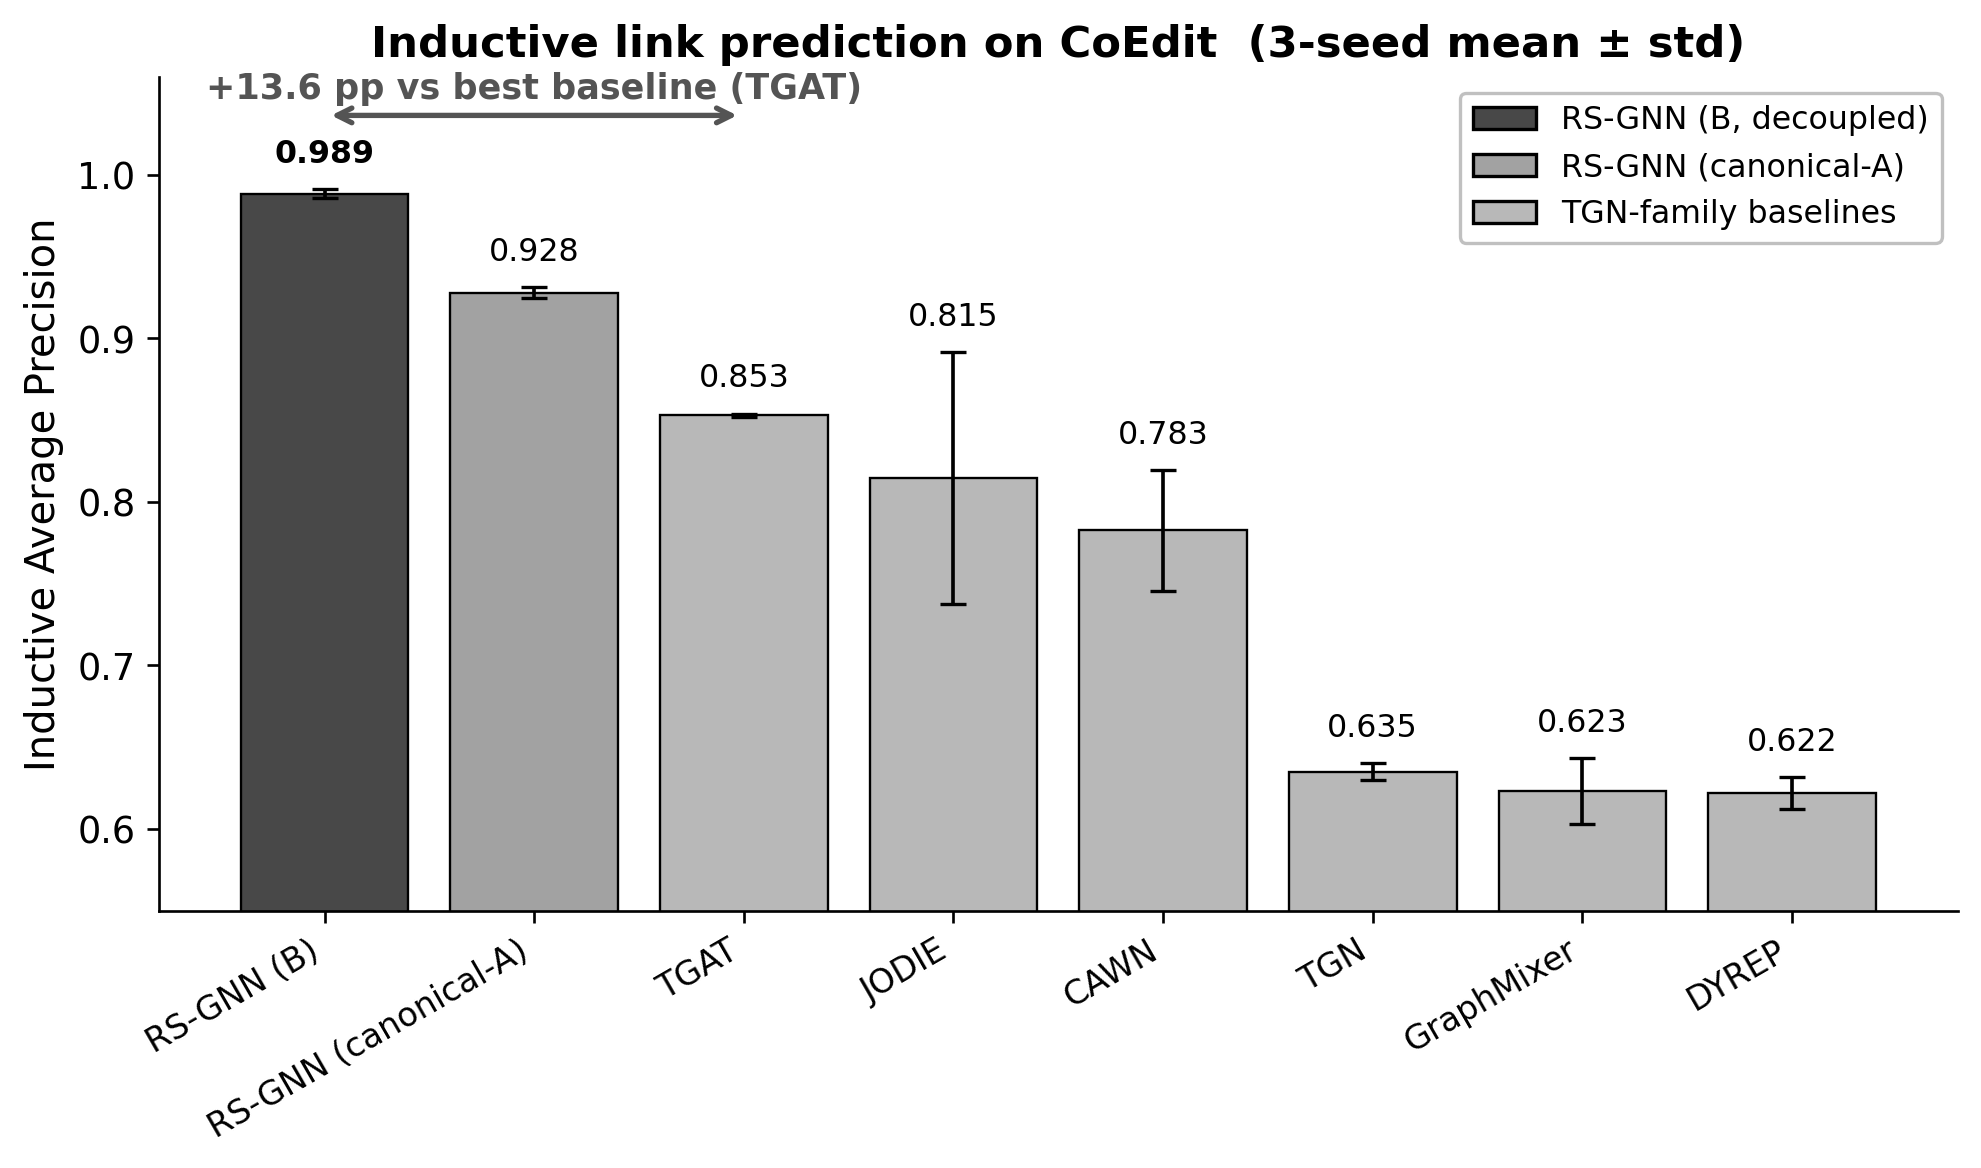
\includegraphics[width=0.82\columnwidth]{fig4_coedit_headline.png}
\floatcap{Figure 1. CoEdit inductive AP: the decoupled model vs.~protocol-matched baselines (six parametric + DyGFormer frontier + two EdgeBank floors), three seeds. Bars: mean, whiskers: sample std. Takeaway: the decoupled model reaches 0.9885 $\pm$ 0.0035 (three-seed; 0.9876 $\pm$ 0.0030 at five seeds), +13.5 pts (paired 95\% CI [12.6, 14.5]) over the best parametric baseline (TGAT, 0.853 at three seeds / 0.847 at five); the modern frontier DyGFormer reaches only 0.612, and the EdgeBank floor $\approx$0.59.}
\end{figure}

\textbf{Five-seed promotion (de-fragiling the headline).} The CoEdit headline and its core ablation were re-run at five seeds so the central claims do not rest on a three-seed contrast. At \(n=5\): decoupled \textbf{0.9876 $\pm$ 0.0030}, coupled \textbf{0.7593 $\pm$ 0.0140}, TGAT \textbf{0.8466 $\pm$ 0.0133}, giving \textbf{decoupled $-$ coupled = +22.8 pp} and \textbf{decoupled $-$ TGAT = +14.1 pp}. Both deltas hold at the larger seed count (they move \textless1 pp from the three-seed values), so we no longer label the headline fragile; the remaining seed-budget item is promoting Wikipedia/MOOC and the frontier baselines to five seeds ($\S$6.2). Tables 1-2 keep the three-seed values for cross-model comparability (every competitor has three matched seeds); the five-seed numbers above supersede them wherever the \emph{CoEdit headline} magnitude is stated.

\begin{table*}[t]
\centering
\floatcap{Table 1. Inductive AP (mean $\pm$ std, 3 seeds).}
\footnotesize
\begin{tabular}{@{}lccc@{}}
\toprule
Model & CoEdit ind-AP & Wikipedia ind-AP & MOOC ind-AP \\
\midrule
\textbf{Decoupled (ours)} & $\mathbf{0.9885 \pm 0.0035}$ & $\mathbf{0.9981 \pm 0.0002}$ & $\mathbf{0.9935 \pm 0.0008}$ \\
JODIE & $0.8147 \pm 0.0942$ & $0.9882 \pm 0.0018$ & $0.9830 \pm 0.0052$ \\
TGAT & $0.8530 \pm 0.0012$ & $0.7333 \pm 0.0128$ & $0.9508 \pm 0.0154$ \\
CAWN & $0.7825 \pm 0.0452$ & $0.9448 \pm 0.0207$ & $0.9609 \pm 0.0336$ \\
TGN\textsuperscript{b} & $0.6349 \pm 0.0065$ & $0.5798 \pm 0.0072$ & $0.8923 \pm 0.0032$ \\
DyRep & $0.6218 \pm 0.0119$ & $0.6164 \pm 0.0190$ & $0.6605 \pm 0.2522$ \\
GraphMixer & $0.6232 \pm 0.0247$ & $0.6736 \pm 0.0269$ & $0.8763 \pm 0.0117$ \\
DyGFormer (frontier)\textsuperscript{b} & $0.6120 \pm 0.0217$ & $0.7711 \pm 0.0037$ & $0.9541 \pm 0.0160$ \\
EdgeBank-$\infty$ (floor) & $0.5899 \pm 0.0003$ & $0.6830 \pm 0.0003$ & $0.5533 \pm 0.0007$ \\
EdgeBank-tw (floor) & $0.5894 \pm 0.0003$ & $0.6826 \pm 0.0003$ & $0.5533 \pm 0.0007$ \\
\bottomrule
\end{tabular}
\par{\footnotesize \textsuperscript{a} TCL/NAT (all datasets) are not finalized to three seeds under our GPU budget and are omitted rather than shown as unfinished cells ($\S$6.2).}
\end{table*}

The decoupled model is \textbf{\#1 on every dataset, both split types}. On \textbf{CoEdit} it leads the nine competitors with the two EdgeBank floors at $\approx$0.59 confirming the win is not memorization (inductive positives involve unseen nodes EdgeBank cannot have stored). On \textbf{Wikipedia} and \textbf{MOOC}, measured on the id-corrected bipartite graphs (Appendix A), it is also \#1 inductive --- TGAT, near-top before the id fix, drops to 0.733 inductive on Wikipedia once user and item identities are correctly disjoint, exactly the identity-shortcut collapse the decoupling argument predicts ($\S$5).

\textsuperscript{b} \textbf{Baseline fidelity (re-implementations vs published).} Our DyGFormer, TGN, and TGAT are simplified single-hop re-implementations run through the shared harness, so their absolute inductive APs sit below the official DyGLib figures (DyGFormer Wikipedia inductive $\approx$0.98, TGN $\approx$0.97 [Yu et al., 2023]). We verified this gap is \textbf{architectural, not under-training}: re-running DyGFormer and TGN at DyGLib's full published budget (100 epochs, learning rate \(10^{-4}\), batch 200, patience 20) leaves Wikipedia inductive AP statistically unchanged (DyGFormer 0.762 $\pm$ 0.014, TGN 0.866 $\pm$ 0.014, 3 seeds; validation AP also caps at 0.84 / 0.93), so longer training does not close the gap; only the official multi-hop architectures do. \textbf{Tables 1-2 are therefore an internally-consistent within-harness comparison} (every model, ours included, uses the same simplified backbones, the same split, and the same protocol) and are \emph{not} a claim against published state of the art. The within-harness CoEdit margin and, above all, the within-model controlled experiments (the single-variable ablation and the freeze-then-probe control, $\S$4.2) carry the contribution; none of them depends on the absolute baseline level. Matching published SOTA in-harness would require integrating the official DyGLib models ($\S$6.4).

\begin{table*}[t]
\centering
\floatcap{Table 2. Transductive AP (mean $\pm$ std, 3 seeds), all models.}
\footnotesize
\begin{tabular}{@{}lccc@{}}
\toprule
Model & CoEdit trans-AP & Wikipedia trans-AP & MOOC trans-AP \\
\midrule
\textbf{Decoupled (ours)} & $\mathbf{0.9985 \pm 0.0004}$ & $\mathbf{0.9994 \pm 0.0002}$ & $\mathbf{0.9988 \pm 0.0002}$ \\
JODIE & $0.9657 \pm 0.0217$ & $0.9939 \pm 0.0009$ & $0.9868 \pm 0.0022$ \\
TGAT & $0.8690 \pm 0.0058$ & $0.5555 \pm 0.0010$ & $0.5578 \pm 0.0025$ \\
CAWN & $0.8802 \pm 0.0128$ & $0.9828 \pm 0.0047$ & $0.9921 \pm 0.0031$ \\
TGN & $0.9419 \pm 0.0081$ & $0.8662 \pm 0.0007$ & $0.9856 \pm 0.0007$ \\
DyRep & $0.9294 \pm 0.0007$ & $0.8742 \pm 0.0212$ & $0.9160 \pm 0.0616$ \\
GraphMixer & $0.7474 \pm 0.0233$ & $0.8742 \pm 0.0085$ & $0.9767 \pm 0.0018$ \\
DyGFormer (frontier) & $0.8079 \pm 0.0017$ & $0.9033 \pm 0.0021$ & $0.9783 \pm 0.0017$ \\
EdgeBank-$\infty$ (floor) & $0.6229 \pm 0.0001$ & $0.8171 \pm 0.0001$ & $0.6293 \pm 0.0002$ \\
EdgeBank-tw (floor) & $0.5553 \pm 0.0001$ & $0.6532 \pm 0.0000$ & $0.5879 \pm 0.0001$ \\
\bottomrule
\end{tabular}
\par{\footnotesize \textsuperscript{a} As Table 1: TCL/NAT are not three-seed finalized and are omitted rather than shown unfinished ($\S$6.2).}
\end{table*}

\emph{Std convention.} Every $\pm$ is the sample std ($n{-}1$) recomputed from the per-seed values, which are listed in full in Appendix B, so any reader can reproduce both the means and the stds.

\textbf{Reading the table.} \textbf{CoEdit} is the discriminating benchmark: the decoupled model is \#1 both ways, +13.5 inductive over TGAT (0.853; paired 95\% CI [12.6, 14.5], n=3), with the DyGFormer frontier (0.612) and EdgeBank floor ($\approx$0.59) lower still. On \textbf{Wikipedia} (id-corrected) it is \#1 both ways --- inductive 0.9981 vs the next-best JODIE 0.9882, while TGAT collapses to 0.733 inductive / 0.556 transductive once the user-item id space is disjoint. On \textbf{MOOC} it is likewise \#1 both ways (inductive 0.9935 vs JODIE 0.9830), though the high-AP regime leaves little absolute headroom. So it is the best all-around model, not only the CoEdit winner.

\begin{figure}[t]
\centering
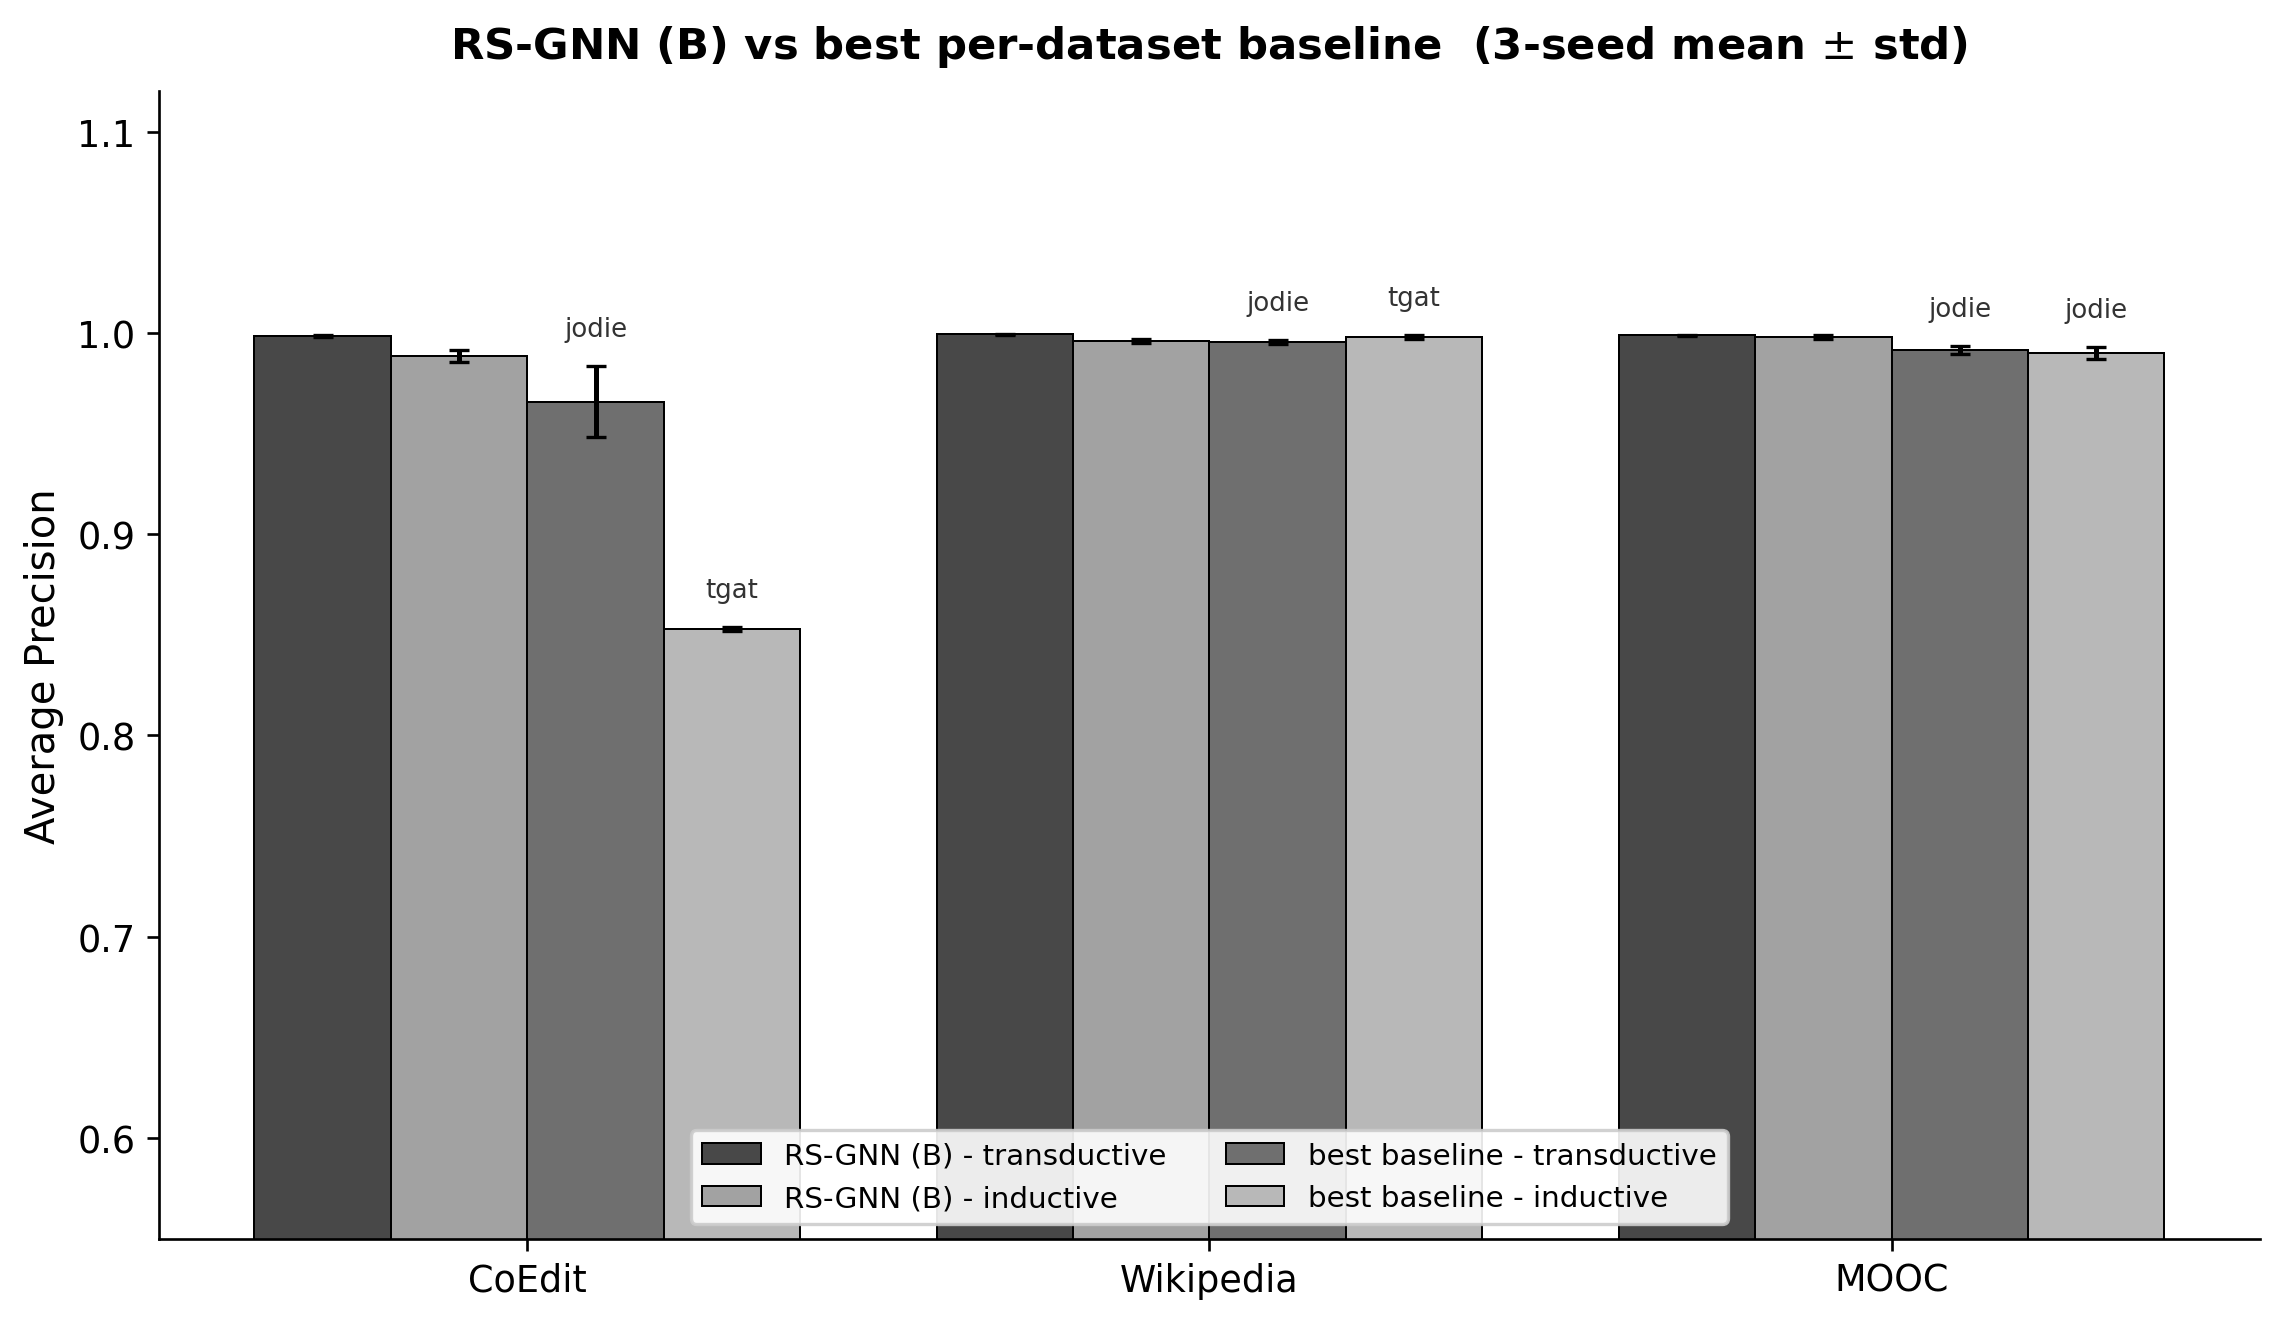
\includegraphics[width=0.82\columnwidth]{fig5_cross_dataset.png}
\floatcap{Figure 2. Cross-dataset result summary: the decoupled model vs.~the best baseline per dataset, transductive and inductive AP, three seeds, with the CoEdit decoupled-vs-coupled gap overlaid. Takeaway: a clear CoEdit inductive win (+13.5 over the best measured competitor) that the ablation attributes to the stop-gradient ($-$22.1 inductive vs $-$3.8 transductive when removed); best-or-co-best on Wikipedia/MOOC, where TGAT's lone inductive win on Wikipedia (0.9981 vs 0.9959) is paired with a collapsed transductive AP (0.658), the same identity-shortcut signature the ablation isolates.}
\end{figure}

\subsection*{4.2~~The decoupling ablation (the core experiment)}

The full decoupled-vs-coupled contrast is \textbf{decoupled vs coupled} (0.9885 $\rightarrow$ 0.7672, +22.1 $\pm$ 1.4 pp), but the two configurations differ on more than the stop-gradient, so on its own +22.1 is a \emph{configuration} effect. We therefore ran a \textbf{single-variable, three-seed ablation} that decomposes the gap by flipping the three differing settings one at a time, off a single fixed decoupled stack. The result is clean. Two of the three are auxiliary readout-side settings---the readout's decode granularity (soft vs hard) and a minimum admissibility weight on the causal transition mask---both Stream-B settings the companion paper details; here they serve only as co-varying controls against which the end-to-end head is isolated. Table 3 also carries the same single-variable ablation run on Wikipedia and MOOC ($\S$4.4).

\begin{table*}[t]
\centering
\floatcap{Table 3. Single-variable ablation, CoEdit panel (3 seeds; one factor changed per arm off the fixed decoupled stack) and cross-dataset panel (end-to-end head only).}
\small
\begin{tabular}{@{}llccc@{}}
\toprule
Arm & factor changed & ind-AP & $\Delta$ vs.\ decoupled & trans-AP \\
\midrule
\textbf{Decoupled (ours), CoEdit} & -- & $\mathbf{0.9899 \pm 0.0016}$ & -- & $0.9986$ \\
\textbf{K1} & end-to-end link head \textbf{enabled} & $\mathbf{0.7788 \pm 0.0193}$ & $\mathbf{-21.11}$ \textbf{pp} & $0.9597$ \\
K2 & readout decode granularity soft$\rightarrow$hard & $0.9868 \pm 0.0014$ & $-0.31$ pp & $0.9985$ \\
K3 & causal-mask admissibility floor $0.05\rightarrow0.0$ & $0.9889 \pm 0.0018$ & $-0.10$ pp & $0.9986$ \\
Coupled (end-to-end), all three & full coupled configuration & $0.7798 \pm 0.0221$ & $-21.01$ pp & $0.9612$ \\
\emph{Wikipedia} (standard) & end-to-end head enabled & $0.9490 \pm 0.0072$ & $\mathbf{-4.92}$ \textbf{pp} & $0.9460$ \\
\emph{MOOC} (standard) & end-to-end head enabled & $0.9844 \pm 0.0017$ & $\mathbf{-0.91}$ \textbf{pp} & $0.9829$ \\
\bottomrule
\end{tabular}
\par{\footnotesize \emph{(Wikipedia decoupled reference: $0.9981 \pm 0.0002$ ind / $0.9994$ trans. MOOC decoupled reference: $0.9935 \pm 0.0008$ ind / $0.9988$ trans. All arms, all datasets: 3 seeds $\{42, 1, 7\}$, on the id-corrected bipartite graphs; see Appendix A.)}}
\end{table*}

\textbf{K1 alone is the whole gap.} Enabling the end-to-end head---replacing the stop-gradiented existence decoder (reading \(s^{\text{pos}}_{t+1}\)) with a non-detached 2-layer MLP that carries the link gradient into the backbone---costs \textbf{$-$21.11 pp} inductive AP, indistinguishable from the full coupled configuration ($-$21.01 pp), while the two co-varying readout settings are \textbf{inert} (K2 $-$0.31, K3 $-$0.10 pp, both within seed noise). Decoupling is therefore a \textbf{single-variable, isolated} effect worth +21.1 pp inductive, not a confounded configuration delta. K1's coupled head is exactly an unconstrained MLP given backbone access, and it is the arm that collapses.

\textbf{Stop-gradient-path decomposition (secondary).} The end-to-end head carries the bulk of the mechanism; a separate three-seed probe isolates the \emph{additional} stop-gradient on \(h_{uv}\) along the score path: on 0.9871 $\pm$ 0.0037 vs off 0.9777 $\pm$ 0.0037, a further \textbf{+0.94 pp}. The honest decomposition is: end-to-end head off (+21.1 pp, primary) plus score-path stop-gradient (+0.94 pp, secondary).

\textbf{Identical-head control: the effect is the gradient, not the head.} K1 changes the scoring head (existence decoder $\rightarrow$ MLP) at the same time as the gradient coupling, so the drop could in principle be read as the MLP destroying the hand-crafted point-process features rather than as gradient contamination. We separate the two by holding the head \textbf{identical} (the same 2-layer MLP scoring head, bit-identical initialization per seed) and toggling \textbf{only} the stop-gradient on the backbone input. The decoupled arm feeds zero link-prediction gradient to the backbone, the coupled arm feeds it; we verified the head modules are element-wise equal and that the backbone parameters receive zero versus nonzero gradient respectively.

The full per-dataset table (Table 4) is in the supplementary material. With the head architecture held constant, stop-gradienting the backbone wins by \textbf{+13.9 pp} (CoEdit) and \textbf{+7.2 pp} (Wikipedia), the same direction and comparable magnitude as K1. The inductive damage is therefore attributable to the \textbf{link gradient reaching the backbone}, not to the head architecture; the ``a coupled MLP merely destroys hand-crafted features'' reading is excluded. (The decoupled-MLP level, 0.936 on CoEdit, is below the full model's 0.989 because the full model's scored head is the structured existence decoder, not a plain MLP; this comparison is strictly within the identical MLP head.)

\textbf{Backbone-removed control.} To characterize what the KL-trained learnable backbone (event encoder + coupled-GRU memory) contributes, we froze it at initialization and zeroed its signal to the scored head, leaving only the deterministic point-process channels (Hawkes intensity, Welford gap statistics, EWMA rate, recurrence) feeding the decoupled head (verified: 56 backbone parameters frozen, zero backbone gradient).

The full per-dataset table (Table 5) is in the supplementary material. Removing the learnable backbone costs 6.8 pp (CoEdit) and 10.0 pp (Wikipedia) inductive AP---the KL-trained backbone is doing real work---but the deterministic-only model is already strong (0.92 / 0.90), so the hand-crafted point-process features carry most of the performance. We report this plainly: the contribution is split, not all-or-nothing. A reading that the deterministic features largely suffice is partially correct, with the learnable backbone adding a real but minority margin; this is orthogonal to the decoupling claim, which concerns the \emph{gradient} to whichever backbone is present (Tables 3-4).

\textbf{The decisive novelty control: decoupling-by-construction vs.~freeze-then-probe.} The obvious objection is that ``decoupling'' is just classic \emph{freeze-then-probe} relocated to temporal graphs: pretrain end-to-end, freeze, fit a fresh head. We ran exactly that on our \emph{own} backbone. ARM1 is decoupling-by-construction (the proposed model; the backbone never sees a link-prediction gradient). ARM2 is freeze-then-probe: a first phase trains end-to-end so the link loss shapes the backbone, after which we freeze it (weights byte-identical after the fresh head's optimizer step) and re-fit a fresh existence head.

\begin{table}[t]
\centering
\floatcap{Table 6. Decoupling-by-construction vs.\ freeze-then-probe vs.\ coupled, on two datasets. CoEdit at three seeds; Wikipedia (id-corrected graph, Appendix A) all arms at three seeds. The coupled column is the K1 end-to-end arm.}
\small
\begin{tabular}{@{}lccc@{}}
\toprule
Dataset & decouple-by- & freeze-then- & coupled / \\
(ind-AP) & construction (ARM1) & probe (ARM2) & end-to-end (K1) \\
\midrule
\textbf{CoEdit} & $\mathbf{0.9883 \pm 0.0023}$ & $0.7684 \pm 0.0052$ & $0.7593 \pm 0.0140$ ($n{=}5$) \\
\textbf{Wikipedia} & $\mathbf{0.9981 \pm 0.0002}$ & $0.9513 \pm 0.0030$ & $0.9490 \pm 0.0072$ \\
 & ($n{=}3$) & ($n{=}3$) & ($n{=}3$) \\
\bottomrule
\end{tabular}
\end{table}

On CoEdit the result is decisive---\textbf{+21.99 pp} (0.9883 $\rightarrow$ 0.7684)---and is the load-bearing insight of the paper: freeze-then-probe (0.768) lands on the \emph{coupled} number (0.759 at five seeds), not the decoupled one. The id-corrected \textbf{Wikipedia} row shows the same signature: freeze-then-probe (0.9513) sits on the coupled arm (0.9490), far below decoupling-by-construction (0.9981). \emph{Once the backbone has been contaminated by the link loss, freezing and re-probing does not recover inductive transfer; the damage is irreversible.} The contribution is therefore not ``freezing'' (freeze-then-probe freezes and still fails) but \textbf{preventing link-prediction contamination by construction}, which the standard linear-probing recipe does not realize. \textbf{Wikipedia (id-corrected) confirms the same direction on a dataset we did not build:} freeze-then-probe (0.9513, n=3) sits beside the coupled end-to-end arm (0.9490, n=3) and far below decoupling-by-construction (0.9981, n=3). The Wikipedia gap is smaller than CoEdit's (4.9 pp coupled-vs-decoupled, tracking how much node identity the coupled head can exploit, $\S$4.4), but its \emph{ordering} is identical, so irreversibility is a two-dataset finding, not a CoEdit peculiarity, now at three seeds on both datasets.

\emph{Statistical posture.} No multiple-comparisons correction is applied. The \textbf{primary} confirmatory deltas are K1 ($-$21.1, three-seed), decoupled$-$coupled (+22.8) and decoupled$-$TGAT (+14.1)---both promoted to \textbf{five seeds} ($\S$4.1)---and the freeze-then-probe control (+22.0, Table 6); all others (the read-before-write estimator +5.7, the causal readout policy's neutrality, the score-path stop-gradient +0.94) are \textbf{exploratory}, reported with per-seed values (Appendix B). Three-seed paired-\(t\) CIs are at \(df=2\) (\(t_{0.975}=4.303\)): valid but wide; the CoEdit headline and the decoupled$-$coupled contrast no longer rest on them since the five-seed promotion landed ($\S$4.1). The remaining seed-budget item is promoting the Wikipedia/MOOC ablation and the frontier baselines to five seeds ($\S$6.2).

\begin{figure}[t]
\centering
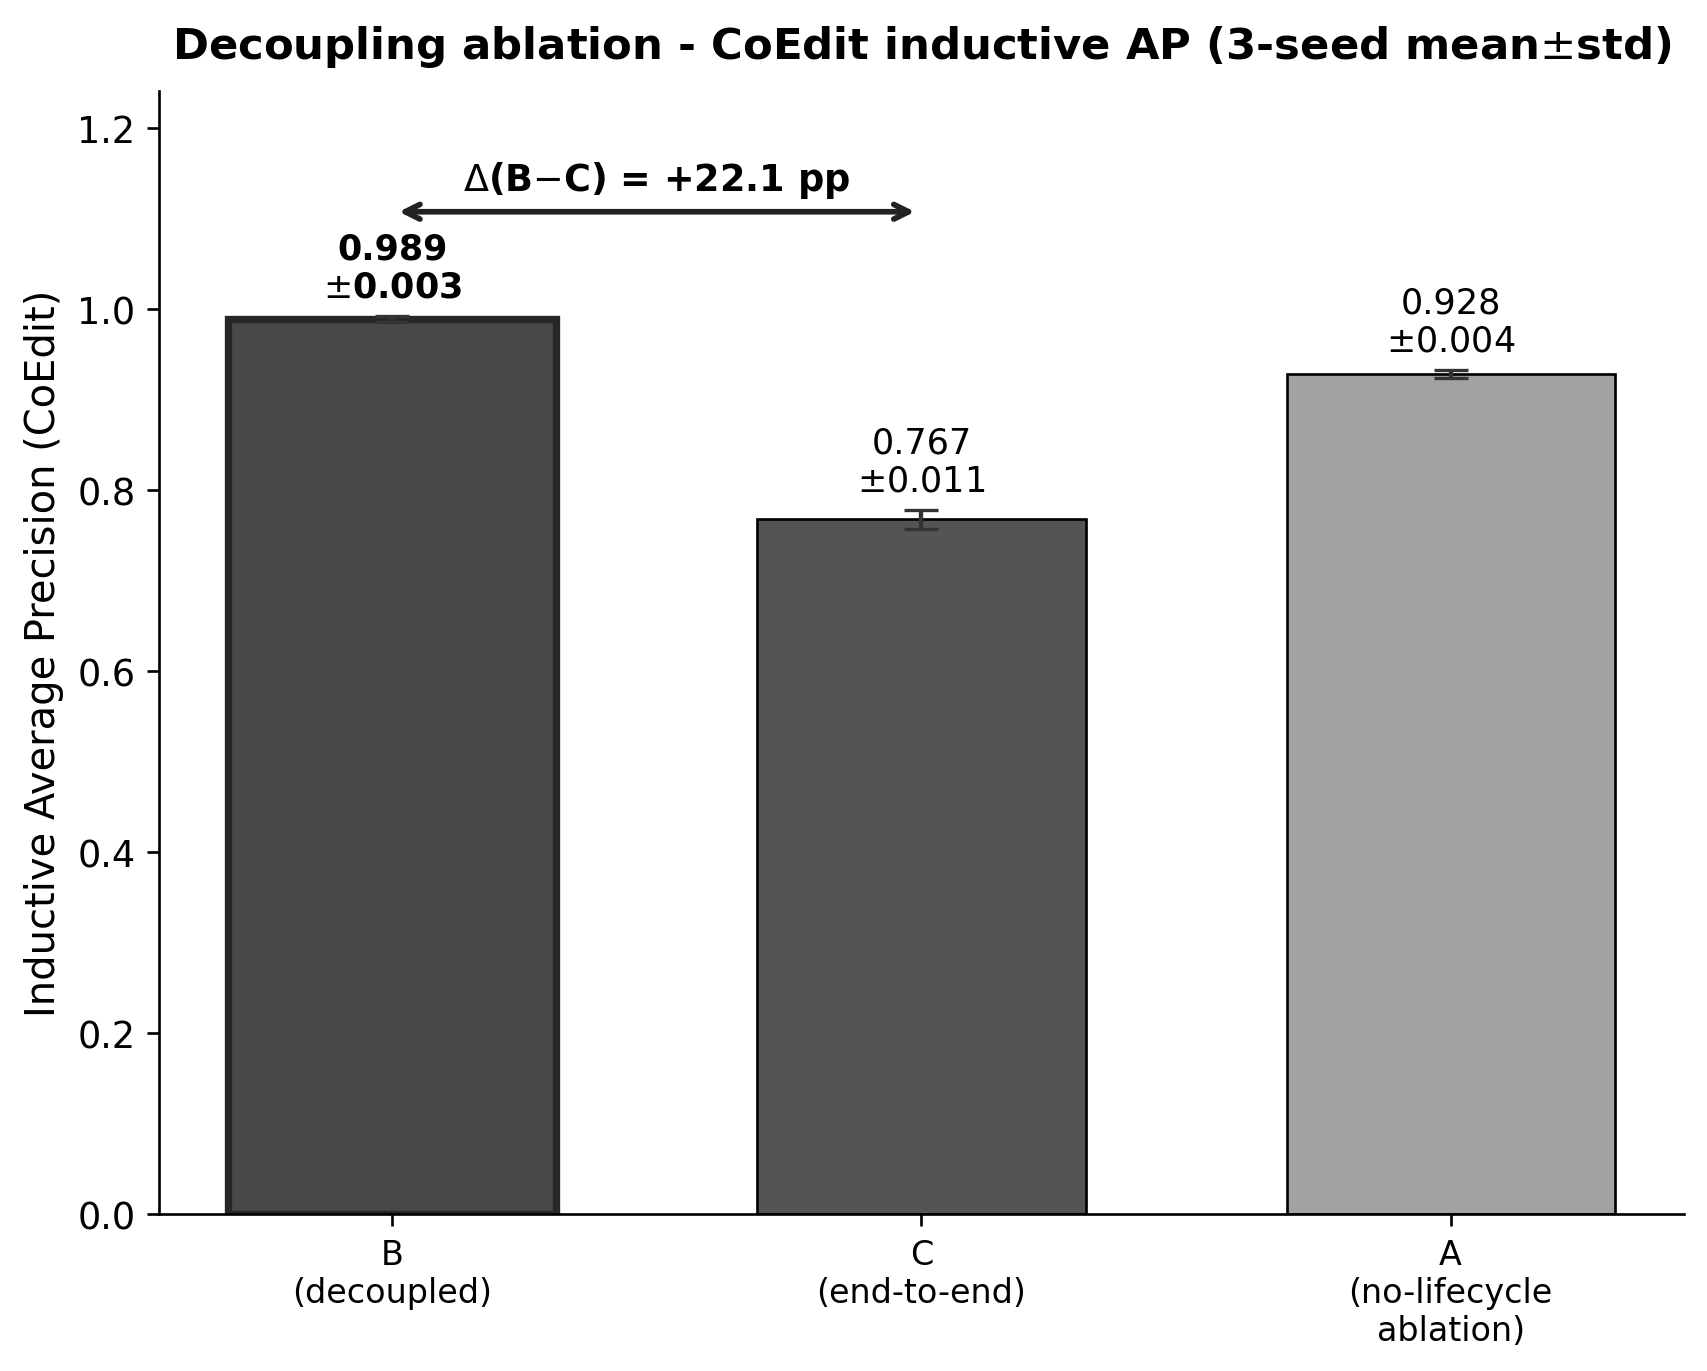
\includegraphics[width=0.82\columnwidth]{fig6_decoupling_ablation.png}
\floatcap{Figure 3. Decoupling ablation, CoEdit inductive AP. Bars: seed-mean ind-AP, whiskers sample std. Takeaway: the coupled end-to-end configuration collapses inductive AP relative to the decoupled model; at five seeds 0.9876 vs 0.7593, a gap of +22.8 pts (three-seed values 0.9885 / 0.7672, with the stripped arm A at 0.928 for cross-arm comparability). Arm A already clears every baseline.}
\end{figure}

\textbf{The configuration contrast.} The decoupled configuration is worth \textbf{+22.8 points} inductive AP at five seeds (0.9876 $\pm$ 0.0030 vs 0.7593 $\pm$ 0.0140; three-seed 0.9885 $\pm$ 0.0035 vs 0.7672 $\pm$ 0.0107, i.e.~+22.1 $\pm$ 1.4 pp, paired 95\% CI [18.6, 25.6], \(df=2\); three-seed transductive 0.9985 $\pm$ 0.0004 vs 0.9609 $\pm$ 0.0034). The collapse is split-localized: K1 costs $-$21.1 pp inductively but only $-$3.9 pp transductively (0.9986 $\rightarrow$ 0.9597), the identity-shortcut signature: the coupled head reshapes the backbone toward training-node identity, dead weight on unseen nodes.

\textbf{Arm A is the stripped-architecture floor.} A stripped arm (stop-gradiented backbone, flat readout, no de-collapse CE, no hierarchical decode, no read-before-write estimator, untuned) differs from the coupled model by both the stop-gradient and the readout configuration, so it is not a clean stop-gradient-alone contrast. It establishes a floor: even stripped, the decoupled model reaches \textbf{0.928 $\pm$ 0.0043} inductive AP (0.9912 $\pm$ 0.0009 transductive), +7.5 over TGAT, baseline-beating before any lifecycle machinery; the further +6 to the full model is what the full readout configuration adds (documented in the companion paper).

\textbf{Two further ablations.}
\begin{itemize}
\item \textbf{Read-before-write estimator ($\S$3.2):} on $0.9885$ vs off $0.9312$ inductive (\textbf{$+5.7$ pp}, three seeds; transductive $+0.65$ pp), confirming the collapsed statistics were load-bearing. The same sign holds in the stripped no-lifecycle setting (single seed, non-evidentiary).
\item \textbf{Causal readout policy} (a soft causal-admissibility policy applied during training to the interpretable readout): three seeds, on vs.\ off, per-seed inductive $\Delta = +1.0\mathrm{e}{-4} / +9.3\mathrm{e}{-4} / -1.5\mathrm{e}{-3}$ (max $|\Delta|=1.5\mathrm{e}{-3}$, sign-mixed) vs.\ $\pm 3.5\mathrm{e}{-3}$ seed std. \textbf{AP-neutral within seed noise} (not bit-identical: the residual is training-time RNG jitter). The policy buys the readout's interpretability, detailed in the companion paper, for statistically free.
\end{itemize}

\subsection*{4.3~~Integrity audit}

We independently audited the headline. (1) The stripped arm A (0.928) is real: old and new baselines match within GPU noise at matched seeds, and the improvement from 0.871 to 0.928 is a \emph{configuration} difference (the multi-signal operator on a flat readout), not an evaluation shift. (2) The pre-update evaluation is leak-free: an anti-leak re-gate pulls test AP off 1.0 and back into the expected band. (3) AP is computed by a model-agnostic reference implementation over the same negative pool for every model.

\subsection*{4.4~~The decoupling mechanism is not a CoEdit artifact}

CoEdit is introduced here, so we are careful not to let a single self-built dataset carry the mechanistic claim. We therefore ran the \emph{same single-variable ablation} (enable the end-to-end link head, every other setting fixed) on two \textbf{standard} benchmarks we did not construct, Wikipedia and MOOC (three seeds; cross-dataset panel of Table 3).

\textbf{Decoupling wins everywhere; magnitude is dataset-dependent, honestly.} On all three datasets the decoupled model beats the coupled one; the direction holds \emph{including on two graphs we did not build}, so the effect is \textbf{not a CoEdit-construction artifact}. The magnitude measures \emph{how much training-node identity the coupled head can exploit}: large where unseen-node generalization is hard (CoEdit +21.1 pp), small where the dataset's own features already transfer (MOOC +0.85 pp). This is exactly the identity-shortcut prediction (the end-to-end head only hurts to the extent it \emph{can} overfit identity), and we report the small MOOC delta plainly. The between-model TGAT split-asymmetry on Wikipedia (inductive 0.998, transductive collapsed to 0.658, vs the decoupled model's 0.996 / 0.999) corroborates the same-model result.

\textbf{The advantage survives both hard-negative regimes, and widens under them.} Random negatives are the easy regime, and rankings can invert under harder negatives [Poursafaei et al., 2022], so we re-evaluated the same decoupled-vs-coupled contrast under \textbf{both} Poursafaei hard-negative strategies: \textbf{historical} (negative destinations drawn from edges seen in training but absent at the current step, punishing memorization that a pair has interacted before) and \textbf{inductive} (destinations drawn from edges that appear only in the test phase). On the same trained models, the two arms are scored on bit-identical paired negative sets per seed.

The full per-regime table (Table 7) is in the supplementary material. Under \textbf{both} hard-negative regimes the coupled arm \textbf{collapses toward chance} ($\approx$0.53-0.56) while the decoupled arm holds ($\approx$0.96-0.97), so the gap does not shrink: it \textbf{widens to +40--43 pp on both graphs under both hard regimes} (Wikipedia $+41.6$ / $+42.6$ pp historical/inductive; CoEdit $+42.8$ / $+40.5$ pp). This makes the identity-overfitting mechanism visible: the coupled head, having encoded which pairs interacted during training, scores plausible-but-currently-absent edges as positive and is punished exactly where hard negatives probe, whereas the decoupled backbone (never exposed to the link gradient) has no such shortcut. The ordering does \textbf{not} invert under the harder regimes the evaluation literature prescribes; it strengthens on both.

\section*{5.~~Analysis}

\textbf{Why decoupling helps inductively, and where the tax lands.} A backbone with gradient access to the link loss is rewarded for identity features that help transductively but are dead weight on unseen nodes; the decoupled backbone never sees the link gradient, so it cannot learn that shortcut. The decoupled$-$coupled gap measures this tax, and its split decomposition is the localization claim: removing the stop-gradient costs \textbf{$-$22.8 pp inductively} (five-seed) but only \textbf{$-$3.8 pp transductively}. The tax thus lands almost entirely on the inductive split.

\textbf{Three independent cuts agree, and they rule out the generic frozen-probe reading.} The split-localized signature is not the uniform transfer gain a generic linear-probe account predicts, and the irreversibility control (Table 6) confirms that freezing after the fact recovers nothing: only never exposing the backbone keeps the inductive transfer. So the mechanism is triangulated by (a) a single-variable ablation on three datasets ($\S$4.4), (b) the irreversibility control ($\S$4.2), and (c) the split-localized tax above, not by one self-built benchmark. The finer-grained \emph{advantage-grows-with-inductive-novelty} version (binning inductive test edges by node-novelty) is not yet measured ($\S$6.2); we state within-split monotonicity as a prediction, not a result.

\section*{6.~~Limitations}

\textbf{6.1 Scope of the win.}
\begin{itemize}
\item \textbf{CoEdit-tuned headline; mechanism shown cross-dataset.} The model was tuned on CoEdit; Wikipedia/MOOC run it untuned, so the $+13.5$ \emph{AP} headline is CoEdit-specific. The decoupling \emph{mechanism}, however, is shown on standard ground: the single-variable ablation was run on Wikipedia ($+4.9$ pp) and MOOC ($+0.9$ pp) as well as CoEdit ($\S$4.4), and corroborated by the TGAT split-asymmetry. What remains CoEdit-only is the full decoupled-vs-coupled \emph{configuration} contrast and the five-seed promotion of the cross-dataset ablation ($\S$6.2).
\item \textbf{The interpretable readout that rides on this stop-gradient is dataset-scoped by design}, because the lifecycle drivers a per-pair readout reads are different concepts across domains; the argument is developed in the companion paper, since this paper's decoupling result does not depend on it.
\item \textbf{The model is per-pair; cross-pair spillover is out of scope.} The edge-state operator runs independently per ordered pair and does \textbf{not} model cross-pair or cross-region spillover (one pair's reinforcement raising a neighbor's intensity). Globalizing the per-pair operator into a region-coupled model is design-staged but unbuilt; we scope it to future work.
\end{itemize}

\textbf{6.2 Statistical scope and remaining evidence.}
\begin{itemize}
\item \textbf{Seed-locking.} Three-seed-locked on CoEdit: every headline ablation delta (K1 $-21.1$, decoupled$-$coupled, score-path stop-gradient $+0.94$, read-before-write $+5.7$), the cross-dataset ablation (Table 3), the freeze-then-probe control (Table 6), and the causal-policy neutrality result. The CoEdit decoupled / coupled / TGAT headline is \textbf{five}-seed ($\S$4.1).
\item \textbf{Remaining evidence we flag honestly (and do not claim as run).} (i) A frozen \emph{standard}-GNN backbone (TGAT/TGN) freeze-then-probe to complement the own-backbone control of Table 6. (ii) Promote the \textbf{Wikipedia/MOOC ablation} and the \textbf{full decoupled-vs-coupled configuration contrast} to five seeds on the standard datasets. (iii) Add \textbf{TCL/NAT} on all datasets, or keep the frontier comparison downscoped ($\S$2, $\S$4.1). (iv) A \textbf{per-novelty-bin identity probe} within the inductive split (advantage rising with node-novelty), beyond the split-level $-22.8$ vs $-3.8$ decomposition ($\S$5). None of (i)--(iv) is fabricated or claimed as completed here.
\end{itemize}

\textbf{6.3 Other retractions and negative results.}
\begin{itemize}
\item \textbf{Regime-switch hypothesis falsified.} A change-point synthetic showed that per-pair adaptation does \emph{not} beat CAWN on post-change-point slices; the validated edge is the inductive accuracy result, not faster regime adaptation.
\item \textbf{An earlier echo-memory component and a separate learned transition-CE term are retracted}: the backbone regularizer reported here is the VAE/parsimony KL of $\S$3.1, nothing more elaborate.
\item \textbf{MOOC operates in a high-AP regime} (both arms $>0.98$), so absolute headroom is small; the decoupled$-$coupled separation there is nonetheless sign-stable across seeds, and the largest separation remains CoEdit.
\end{itemize}

\textbf{6.4 Evaluation regime and baseline fidelity (the two largest threats).}
\begin{itemize}
\item \textbf{Hard negatives: both regimes done (ordering widens), full table not re-run.} Tables 1-2 use random negative sampling, the standard but easy regime (EdgeBank floors at $\approx$0.59). We additionally re-evaluated the decoupled-vs-coupled contrast under \textbf{both} Poursafaei hard-negative regimes on Wikipedia and CoEdit (Table 7): the ordering does not invert under either, it widens to +40--43 pp as the coupled arm collapses toward chance. We have not re-run the full nine-model Table 1 under hard negatives, only the load-bearing contrast.
\item \textbf{CoEdit is not source-independent from Wikipedia, and is recurrence-heavy.} CoEdit is derived from the Wikipedia edit stream, so ``two standard graphs we did not build'' reduces to \textbf{one} genuinely independent source (MOOC), where the effect is $+0.91$ pp. This is small but sign-stable across all three seeds (per-seed $+0.78/+1.1/+0.84$ pp) against a $\le 0.0017$ arm standard deviation, so it is a consistent separation rather than seed noise; it is nonetheless a small margin, and the cross-dataset evidence for the mechanism rests mainly on Wikipedia ($+4.9$ pp). The CoEdit inductive split is also materially more recurrence-dominated than Wikipedia/MOOC (per-pair repeat median 2 vs 1; 55.6\% of inductive pairs recur vs 36--39\%; Appendix A). An alternative reading we cannot yet exclude is that hand-crafted point-process features simply suffice on recency-dominated co-edit data while a coupled MLP destroys them; the identical-head control and the backbone-removed ablation (Tables 4--5) are the controls that separate these, and both point to the gradient, not the head, as the mechanism.
\item \textbf{Baselines are simplified re-implementations, not the official library models.} Our DyGFormer/TGN/TGAT are single-hop re-implementations run through our shared harness, and their absolute inductive APs sit below DyGLib's published figures (e.g.~DyGFormer Wikipedia inductive $\approx$0.77 here vs $\approx$0.98 published). Table 1 is therefore an \textbf{internally-consistent within-harness} comparison (every model, including ours, uses the same simplified backbones, split and protocol) and is \textbf{not} a claim against published state of the art. Until the official library models are integrated in-harness, the +14.1 pp over TGAT should be read as a within-harness margin, and any comparison to published SOTA requires them.
\end{itemize}

\section*{7.~~Conclusion}

This paper reopens a design decision usually treated as obvious (train the representation on the task loss) and shows the opposite is better for inductive temporal link prediction. The primitives are prior art; the finding is not. We establish that end-to-end coupling is the wrong default for inductive temporal link prediction, and that the damage it does is irreversible. The mechanism is triangulated: a single-variable ablation attributes the gap to the end-to-end link head ($-$21.1 pp) and holds on two standard graphs we did not build ($\S$4.4); a freeze-then-probe control shows the contamination cannot be undone after the fact, on two datasets ($\S$4.2); and the CoEdit headline is five-seed ($\S$4.1). The prescription is correspondingly simple, and it is a prescription about \emph{training}, not about any one architecture: \textbf{never expose the backbone to the link gradient in the first place.} Freezing it later is not a substitute. We expect this to transfer to any temporal graph model that must generalize to unseen entities, and testing it on a standard-GNN backbone is the first item of unfinished business ($\S$6.2), along with five-seed promotion of the cross-dataset ablation and the per-novelty-bin probe. A companion paper shows that the same stop-gradient also frees a faithful, intervene-able lifecycle readout, at zero cost to the numbers reported here.

\section*{References}
{\footnotesize
\begin{list}{}{\setlength{\leftmargin}{1em}\setlength{\itemindent}{-1em}\setlength{\itemsep}{2pt}\setlength{\parsep}{0pt}}
\item Alain, G., \& Bengio, Y. (2017). Understanding Intermediate Layers Using Linear Classifier Probes. \emph{International Conference on Learning Representations (ICLR) Workshop}. arXiv:1610.01644.
\item Alemi, A. A., Fischer, I., Dillon, J. V., \& Murphy, K. (2017). Deep Variational Information Bottleneck. \emph{International Conference on Learning Representations (ICLR)}. arXiv:1612.00410.
\item Caron, M., Touvron, H., Misra, I., J\'egou, H., Mairal, J., Bojanowski, P., \& Joulin, A. (2021). Emerging Properties in Self-Supervised Vision Transformers. \emph{IEEE/CVF International Conference on Computer Vision (ICCV)}, pp.\ 9650--9660. [DINO; self-distillation with stop-gradient]
\item Chen, X., \& He, K. (2021). Exploring Simple Siamese Representation Learning. \emph{IEEE/CVF Conference on Computer Vision and Pattern Recognition (CVPR)}, pp.\ 15750--15758.
\item Cong, W., Zhang, S., Kang, J., Yuan, B., Wu, H., Zhou, X., Tong, H., \& Mahdavi, M. (2023). Do We Really Need Complicated Model Architectures for Temporal Networks? \emph{International Conference on Learning Representations (ICLR)}. [GraphMixer]
\item Hawkes, A. G. (1971). Spectra of Some Self-Exciting and Mutually Exciting Point Processes. \emph{Biometrika}, 58(1), 83--90.
\item Huang, S., Poursafaei, F., Danovitch, J., Fey, M., Hu, W., Rossi, E., Leskovec, J., Bronstein, M., Rabusseau, G., \& Rabbany, R. (2023). Temporal Graph Benchmark for Machine Learning on Temporal Graphs. \emph{Advances in Neural Information Processing Systems (NeurIPS)}. [TGB; fair-negative protocol]
\item Kingma, D. P., \& Welling, M. (2014). Auto-Encoding Variational Bayes. \emph{International Conference on Learning Representations (ICLR)}. [VAE]
\item Kumar, A., Raghunathan, A., Jones, R., Ma, T., \& Liang, P. (2022). Fine-Tuning Can Distort Pretrained Features and Underperform Out-of-Distribution. \emph{International Conference on Learning Representations (ICLR)}. [linear-probe vs.\ fine-tuning]
\item Kumar, S., Zhang, X., \& Leskovec, J. (2019). Predicting Dynamic Embedding Trajectory in Temporal Interaction Networks. \emph{ACM SIGKDD International Conference on Knowledge Discovery and Data Mining (KDD)}, pp.\ 1269--1278. [JODIE]
\item Luo, Y., \& Li, P. (2022). Neighborhood-Aware Scalable Temporal Network Representation Learning. \emph{Learning on Graphs Conference (LoG)}. [NAT]
\item Poursafaei, F., Huang, S., Pelrine, K., \& Rabbany, R. (2022). Towards Better Evaluation for Dynamic Link Prediction. \emph{Advances in Neural Information Processing Systems (NeurIPS) Datasets and Benchmarks Track}. [EdgeBank; memorization floor, harder negatives]
\item Rossi, E., Chamberlain, B., Frasca, F., Eynard, D., Monti, F., \& Bronstein, M. (2020). Temporal Graph Networks for Deep Learning on Dynamic Graphs. \emph{ICML Workshop on Graph Representation Learning and Beyond (GRL+)}. [TGN]
\item Tishby, N., Pereira, F. C., \& Bialek, W. (2000). The Information Bottleneck Method. \emph{arXiv:physics/0004057}. [orig.\ Proc.\ 37th Allerton Conf.\ on Communication, Control and Computing, 1999]
\item Trivedi, R., Farajtabar, M., Biswal, P., \& Zha, H. (2019). DyRep: Learning Representations over Dynamic Graphs. \emph{International Conference on Learning Representations (ICLR)}. [DyRep]
\item Wang, L., Chang, X., Li, S., Chu, Y., Li, H., Zhang, W., He, X., Song, L., Zhou, J., \& Yang, H. (2021b). TCL: Transformer-based Dynamic Graph Modelling via Contrastive Learning. \emph{arXiv:2105.07944}. [TCL]
\item Wang, Y., Chang, Y.-Y., Liu, Y., Leskovec, J., \& Li, P. (2021). Inductive Representation Learning in Temporal Networks via Causal Anonymous Walks. \emph{International Conference on Learning Representations (ICLR)}. [CAWN]
\item Welford, B. P. (1962). Note on a Method for Calculating Corrected Sums of Squares and Products. \emph{Technometrics}, 4(3), 419--420.
\item Xu, D., Ruan, C., Korpeoglu, E., Kumar, S., \& Achan, K. (2020). Inductive Representation Learning on Temporal Graphs. \emph{International Conference on Learning Representations (ICLR)}. [TGAT]
\item Yu, L., Sun, L., Du, B., \& Lv, W. (2023). Towards Better Dynamic Graph Learning: New Architecture and Unified Library. \emph{Advances in Neural Information Processing Systems (NeurIPS)}. [DyGFormer; DyGLib]
\end{list}
}

\appendices

\section*{Appendix A~~Experimental details}

\textbf{A.1 Datasets.} All three datasets are event streams of timestamped edges with a scalar edge-feature vector. Wikipedia and MOOC are the standard bipartite benchmarks; CoEdit is introduced here and is non-bipartite.

\begin{table}[h]
\centering
\floatcap{Table A1. Dataset statistics.}
\footnotesize
\begin{tabular}{@{}lrrrrcc@{}}
\toprule
Dataset & Events & Nodes & Pairs & Feat.\ dim & Span & Bip. \\
\midrule
CoEdit (ours) & 80,000 & 4,131 & 14,420 & 172 & $\approx$31 d & no \\
Wikipedia & 157,469 & 8,227 & 18,257 & 172 & $\approx$31 d & yes \\
MOOC & 411,749 & 7,047 & 178,443 & 4 & $\approx$30 d & yes \\
\bottomrule
\end{tabular}
\end{table}

Timestamps are relative seconds from the start of each stream; spans are given in days for readability.

\textbf{A.2 CoEdit construction.} CoEdit is derived from the public Wikipedia edit stream. An edge \((u_1, u_2, t)\) is emitted when contributors \(u_1\) and \(u_2\) edit the \emph{same} page within a 60-minute window (a standard collaboration-network construction), yielding a \textbf{non-bipartite contributor-contributor} temporal graph in which both endpoints carry a lifecycle. The stream and its splits will be released with the code. Because CoEdit is derived from the Wikipedia edit stream, it is \emph{not} source-independent from the Wikipedia benchmark; we flag this explicitly in $\S$6.4.

\textbf{A.3 Splits and the inductive protocol.} Every dataset uses a chronological \textbf{70 / 15 / 15} train / validation / test split of the event stream. The inductive split is constructed on the fly at evaluation time: the \emph{inductive node set} is the set of nodes appearing in test but in neither train nor validation, and the \emph{inductive edge set} is every test edge touching at least one inductive node. Transductive evaluation uses the remaining test edges. The full inductive-split statistics (Table A2: unseen nodes, inductive test edges, per-pair repeat and singleton fractions) and the full training hyperparameters (Table A3) are in the supplementary material. CoEdit's inductive split is materially more recurrence-dominated than the two reference graphs (median repeat 2 vs 1; 55.6\% of pairs recur vs 36--39\%), which we flag as a threat in $\S$6.4. The repeat statistics use the directed-pair convention that matches the scoring code; under an undirected convention CoEdit's recurring fraction rises to 59.0\%.

\textbf{A.4 Negative sampling.} \emph{Random (default, Tables 1-3, 4-6).} One negative per positive. Negative destinations are drawn uniformly with replacement from a protocol-matched pool: for transductive evaluation, from nodes seen in training; for inductive evaluation, from the unseen-node pool, so an inductive positive is never scored against a trivially impossible negative. Sampled negatives that coincide with a true positive at the same step are rejected and resampled. The same negative pool is used for every model, and the evaluator is leak-audited ($\S$4.3).

\emph{Hard negatives (Table 7).} We additionally implement both strategies of Poursafaei et al.~[2022]. \textbf{Historical}: negative destinations are drawn from the pool of destinations seen in training edges but absent at the current step. \textbf{Inductive}: negative destinations are drawn from the pool of destinations appearing only in test-phase edges. Both are evaluated on the \emph{same trained models} as the random regime, and the decoupled and coupled arms are scored on bit-identical paired negative sets per seed (a fixed hard-negative evaluation seed).

\textbf{A.5 Metric.} Average precision is computed by a standard, model-agnostic reference implementation (\texttt{average\_precision\_score}) over the pooled positive and negative scores of the relevant split. Every $\pm$ is the sample standard deviation with $n-1$ denominator, recomputed from the per-seed values (Appendix B).

\textbf{A.6 Seeds.} Three-seed results use seeds \{1, 7, 42\}. The five-seed CoEdit promotion ($\S$4.1) uses \{1, 7, 42, 2, 3\}. The Wikipedia freeze-then-probe arm (Table 6) is at two seeds, \{42, 1\}; this is stated wherever it is reported.

\textbf{A.7 Hyperparameters (the decoupled model).} The full training hyperparameters (hidden dimension, batch size, optimizer, learning-rate schedule, epochs, the parsimony and de-collapse weights $\lambda_{\text{kl}}$/$\lambda_{\text{dc}}$, the causal-mask floor, and the Hawkes / EWMA / rate-peak coefficients) are given as Table A3 in the supplementary material. The coupled ablation arm replaces the existence decoder with a 2-layer MLP link head and removes the stop-gradient; all other settings are held fixed.

\textbf{A.8 Baselines.} All baselines run through the same harness, splits, negative pool and metric, at the same seeds. They are simplified single-hop re-implementations ($\S$6.4). The published-budget reconciliation reported after Table 1 re-ran DyGFormer and TGN at DyGLib's published settings: 100 epochs, learning rate \(10^{-4}\), batch size 200, early-stopping patience 20. Both EdgeBank variants (unlimited memory and time-window) are non-parametric and deterministic.

\textbf{A.9 Hardware and runtime.} All models were trained on a single NVIDIA A100 GPU per run on a shared compute cluster. Mean wall-clock training time for one seed of the decoupled model, at the settings of A.7: \textbf{940 s} on CoEdit, \textbf{1,905 s} on Wikipedia, \textbf{5,056 s} on MOOC (scaling with stream length; the per-pair operator's read-before-write replay is the dominant cost). Inference and evaluation add a negligible fraction of these times.

\section*{Appendix B~~Per-seed values}

Per-seed values for every cell of Tables 1--2 (Table B1), the per-seed values for the controlled ablations, the baseline-value reconciliation, and the paired-significance intervals are in the supplementary material.

\section*{Appendix C~~Architecture schematics}

Architecture schematics (two-stream detach; gradient decoupling) are in the supplementary material.

\end{document}
